\chapter{Theory}
%PR 3 St 2. Some intro recap motivation
Our goal, is to add the final steps in the theory chain which transforms the GRMHD simulations into interferometric observables. For this to be achieved and for the theory higher up in the chain to be maximally useful in data interpretation, realistic signal corruptions need to be considered. Hence, the purpose of this module is to further the sophistication of the interplay between theory and observation in the field.
%The plan for the chapter? PR 3 St 2
The signal corruptions which we have identified as the most prominent occurs in the troposphere, interstellar medium (ISM) and within the stations themselves. First I will review some EM wave fundamental and introduce scattering theory, which is applicable to both the radiative process occuring in the troposphere and ISM. Following the general introduction I will explore each specific case.

\section{Radio Interferometry}
%PR 2 St 3 Define basic radio interferometry concepts. Reference Thompson, Smirnov
%Visibility, the interferometric measurement i.e. measuring electric field covariance (smirnov_1)
% Define the correlations measured

%UV Sampling, Earth rotation synthesis

% van-citterlike theorem a relationship between the image of the sky and it's fourier transform.

%\begin{equation}\label{eq:vis_im}
%van-citterlike theorem
%\end{equation}•

\subsection{Measurement Equation}\label{sec:RIME}
%PR 2 St 3, reference smirnov
%iniyan has paper coming out with a clear succint explanation

%Follow Smirnov, first RIME paper , Introduce Jones formalism


%DDE vs DIE.. + diagram?

\subsection{A primer on self-calibration}
%Pr 2 St 3

%Why the primer

%calibration in mm-VLBI

%Self-calibration from point of view of RIME

\subsection{mm-VLBI observables and data products}
%PR 2 St 2

%Visibility amplitudes, closure quantities, polarisation ratios, and images.
If the visibility phase is highly variable as in the case of a turbulent atmosphere,  conventional calibration and imaging techniques have severely limited (if any) success. However information can still be extracted from the raw visibilities in the form of closure quantities \citep{Monnier_2007} or polarisation ratios \citep{Fish_2009}. Closure phase, defined as the sum of 3 visibility phases of a triangle of stations $\left\{i,j,k\right\}$, is a probe of asymmetry in source structure,
\begin{equation}
\Phi_{ijk} = \phi_{ij}+\phi_{jk}+\phi_{ki}.
\end{equation}

\noindent Because most signal corruptions are station based, the gain phase terms $\phi_{ij}=\phi^{\rm true}+ \phi^G_i -\phi^G_j$ for each antenna will cancel, yielding a more robust observable. 

The uncertainty on the closure phase is model dependent \citep{Rogers_1995} and is given as a function of the SNR $s$ of each baseline 

\begin{equation}\label{eq:ucp}
u(\Phi_{ijk}) = \frac{\sqrt{4 + (s_{ij}s_{jk})^2 + (s_{jk}s_{ki})^2 + (s_{ij}s_{ki})^2 +
                        2(s_{ij}^2+s_{jk}^2+s_{ki}^2)}}{s_{ij}s_{jk}s_{ki}},
\end{equation}

\noindent where $s_{ij}$ is defined as
\begin{equation}
s_{ij}=|V_{ij}| \sqrt{\frac{ \tau \Delta \nu}{SEFD_i SEFD_j}},
\end{equation}
where $\tau$ is the vector averaging timescale, $\Delta \nu$ is the bandwidth, $|V_{ij}|$ is the visibility amplitude and $SEFD$ is the system equivalent flux density. The result that closure phase is entirely immune to station based effects breaks down however when time averaging in the presence of baseline dependent effects like thermal noise as illustrated in section~\ref{closure_errors}.
 
\subsection{Variability and the static source assumption}
%PR 1 St 1

%the assumption and how it breaks the image-vis fourier transform relation
Implicit in our description of interferometry above, we assumed that the source remains approximately unchanged or static during the course of the observation. However, if this assumption does not hold (i.e. if the source is time-variable),  the visibilities measured over the course of an observation can no longer be related to a single image and if they are, the resulting image would appear smeared out as it is averaged over many realisations. 
%explicitly defining variability as any intrinsic source variability
Note that I am using the term `variability' in a general sense which refers to changes in any source observables. Most commonly variability is refers to changes in source flux (visibility amplitude) but I include changes in source structure and position (visibility phase) and source polarisation. Practically it is difficult to separate source and instrumental variability without accurate models and measurements for all non-source signal propagation effects. 
%Observed variability from SgrA
Although the static source assumption holds for most interferometric observations, the accretion flow and/or magnetic field structures around a SMBH can be variable on far shorter timescales. The primary mm-VLBI target, Sgr~$^\star$,  exhibits variability on timescales of minutes to hours in the radio (including in EHT observations), near-infrared (NIR), and X-ray bands \citep[e.g.][]{Baganoff_2001, Genzel_2003, Yusef-Zadeh_2006, Maronne_2006, Fish_2011, Johnson_2015b}. This wealth of observational data has yielded several answers but the origin of the variability is still highly debated. To explain the observed delays between flares in different frequency bands, an expanding adiabatic plasma model (Marrone, 2008) has been presented however a recent flare observed with the EHT did not exhibit the increase in size expected from an expanding plasma outflow model \cite{Fish_2011}.  Signatures of periodic variability at NIR and x-ray \citep{Genzel_2003; Belanger_2006} have been used to argue for the presence of orbiting hotspots \cite{Doeleman_2009}. As the Innermost Stable Circular Orbit (ISCO) depends on spin of the BH, the spin can be constrain through the detection periodic orbital features. However a longer light curve in the NIR is more representative of a power-law scale variability \cite{Meyer_2008}. These observations point to the possibility of multiple flaring mechanisms. An important mm-VLBI observational result is that variability in the polarisation domain is far more rapid than the total intensity (Johnson 2015b), indicating the presence of highly variable magnetic fields.
%Light crossing analysis
In principle, the variability timescale can be comparable to the period of the Innermost Stable Circular Orbit (ISCO), which for Sgr~A$^\star$, ranges from 4 minutes in the maximally rotating realisation to about half an hour for a non-rotating BH. The ISCO period for M87 is longer on the order of day scales. Considering light crossing times $\Delta t_{\rm cross}$, we can estimate the angular size $\theta$ of the emission region to be of order $\theta \sim \Delta t_{\rm cross} c /D_{\rm src}$, where c is the speed of light and $D_{\rm src}$ is the observer-source distance. Hence for Sgr~$^\star$ at a distance of $8.3$~kpc (Gillessen, 2009), for a flare of duration $ \Delta t_{\rm cross} =10$~min, which corresponds to scales of  $15 R_{\rm Sch}$, further evidence of emission areas close the event horizon.
%There are some ways to track/mitigate variability but this is beyond scope
If a flare is dominated by a localised variable structure, several approaches \citep{Doeleman_2009, Fish_2009b, Johnson_2014} show that EHT can track flaring structures with $\sim 5\ \mu$-arcsec precision using closure quantities and polarimetric ratios which could help map the spacetime around the BH. Alternatively \citet{Lu_2016} show that a gaussian weighting scheme can be applied to mitigate the effects of variability and measure the quiescent structure although approach would downweight the longest baselines. However all of these approaches assume only gaussian thermal noise, guassian-blurring in the ISM and no fringe-fitting errors.

\section{Signal Corruptions}

\subsection{Scattering basics}\label{sec:basic_scat}
%PR 1 St 1

%motivation
Millimetre wavelength radiation originating at the Galactic Centre is repeatedly scattered along the signal path to the Earth-based observer. The first occurrence is due to electron plasma in the interstellar medium (ISM) (\citealt{Bower_2006}, \citealt{Gwinn_2014}), while the second is due to poorly-mixed water vapour in the Earth's troposphere (\citealt*{Carilli_1999}, \citealt*{Lay_1997}). It is essential that the effects of the scattering phenomena are understood for a rigorous calibration and interpretation of data.  Towards this end, simulation modules approximating scattering in both media are implemented in \textsc{MeqSilhouette}. As an introduction to the separate descriptions of each, we review a simple scattering model.

%description of the model
An electro-magnetic wave is scattered when it passes through a medium with refractive index inhomogeneities. Following \citet{Narayan_1992}, this effect can be modeled as a thin screen, located between source and observer planes and orientated perpendicular to the line-of-sight. The screen, indexed by coordinate vector $\mathbf{x}$, adds a stochastic phase $\phi(\mathbf{x})$ to the incoming wave at each point on the screen, yielding a corrugated, outgoing wavefront. We define the Fresnel scale as  $r_{\rm F} = \sqrt{\lambda D_{\rm os}/2\pi}$, where $D_{\rm os}$ is the observer-scatterer distance, or the distance where the geometrical path difference $\frac{2\pi}{\lambda} (D_{\rm os} - \sqrt{D_{\rm os}^2 + r_{\rm F}^2}) =\frac{1}{2}$~rad.

%example calculation
To determine the resultant electric field at a point in the plane of the observer, indexed by coordinate vector $\mathbf{X}$, one has to take into account all possible ray paths from the screen to $\mathbf{X}$. To illustrate the model, a calculation of the scalar electric field generated by a point source, $\psi(\mathbf{X})$ yields the Fresnel-Kirchoff integral \citep*{BORN_1980}
\begin{equation}\label{Fresnel- Kirchoff}
\psi(\mathbf{X}) = C \int_{\rm screen} \exp\left[i\phi(\mathbf{x}) + i \frac{(\mathbf{x}-\mathbf{X})^2}{2 r_{\rm F}}\right]\mathbf{dx},
\end{equation}
where C is a numerical constant.

%define structure function
The statistics of $\phi(\mathbf{x})$ can be described by a power spectrum or equivalently the phase structure function,
\begin{equation}\label{eq:D_phi}
D_\phi (\mathbf{x},\mathbf{x'}) = < \left[ \phi(\mathbf{x} +\mathbf{x'}) - \phi(\mathbf{x})\right]^2 >,
\end{equation}
where $\mathbf{x}$ and $\mathbf{x'} $ represent two points on the screen and $<>$ denotes the ensemble average. 

There is evidence that $D_\phi$ can be reasonably approximated by a power law dependence on the absolute distance $r$ between points on the screen  \citep{Armstrong_1995,carilli_1997}
\begin{equation}
D_\phi (r) =  (r/r_0)^\beta,\qquad r^2 = \mathbf{x}^2 - \mathbf{x'}^2
\label{kolmogorov}
\end{equation}
where $r_{\rm 0}$ is the phase coherence length scale defined such that $D_\phi(r_{\rm 0}) = 1$~rad. 
%kolmogorov turbulence
Kolmogorov turbulence, which describes how kinetic energy injected at an outer length scale $r_{\rm out}$ cascades to increasingly smaller scales until finally dissipated at an inner length scale $r_{\rm in}$, predicts $\beta = 5/3$ in the domain ${r_{\rm in}<<r<<r_{\rm out}}$. This scaling has been demonstrated to be a reasonable approximation for the ISM over scales $r \sim 10^2$~km to $>1$~AU \citep*{Johnson_2015a}, and also for the troposphere with $r< \Delta h$, where $\Delta h$ is the thickness of the turbulent layer \cite{Coulman_1985}. The specifics of the tropospheric model will be explored further in later sections.

%Weak and strong
The two length scales, $r_{\rm F}$ and $r_{\rm 0}$, define the nature of the scattering which is split into the strong and weak regimes, Fig.~ref{fig:scatter}. In weak scattering, $ r_{\rm 0} \gg r_{\rm F}$ and hence by equation\ ~\ref{kolmogorov}, $D_{\phi}(r_{\rm F}) \ll 1$. This implies that most of the radiative power measured on a point $\mathbf{X}$ will originate from a screen area $A_{\rm weak} \approx \pi r_{\rm F}^2$. Whereas in the regime of \emph{strong scattering}, $ r_{\rm 0} \ll r_{\rm F}$ yielding  $D_{\phi}(r_{\rm F}) \gg 1$. This  results in coherent signal propagation onto the point $\mathbf{X}$ from multiple disconnected zones each of area $A_{strong} \approx \pi r_{\rm 0}^2$ \citep{Narayan_1992}. Scattering in the troposphere and ISM fall into the regimes of weak and strong scattering respectively.

%Weak and strong fig
\begin{figure*}
\begin{center}
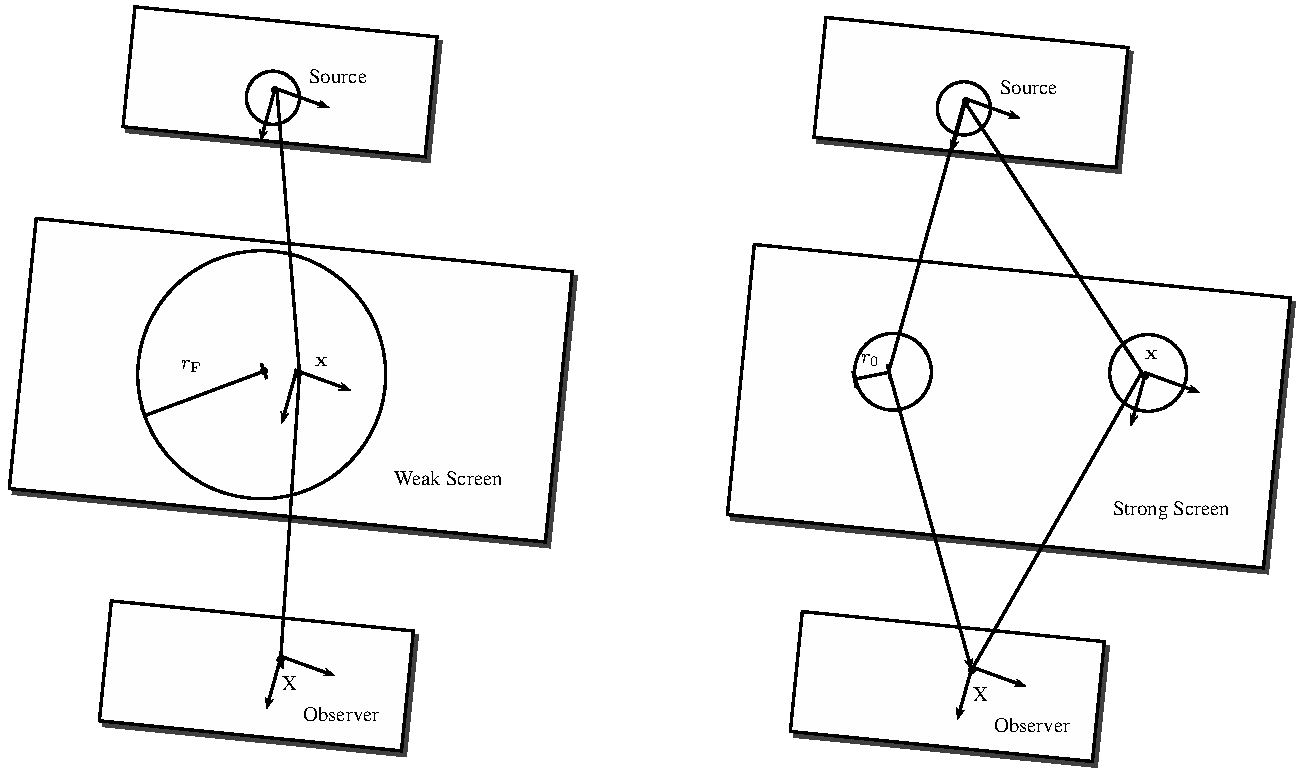
\includegraphics[width=1.\columnwidth]{Images/scatter.pdf}
\caption{Illustration depicting the basics of scattering in the weak (left) and strong (right) regimes. In the weak regime, the signal is coherently propagated over an area, $A_{\rm weak} \approx \pi r_{\rm F}^2$ whereas in the strong regime, coherent propagation is split over many areas of size $A_{strong} \approx \pi r_{\rm 0}^2$. \label{fig:scatter}
}
\end{center}
\end{figure*}

%frozen screen
To evolve the screen in time, we assume a frozen screen i.e. that the velocity of the individual turbulent eddies is dominated by the bulk motion of scattering medium \citep[e.g.][]{Lay_1997}. This allows us to treat the screen as frozen but advected over the observer by a constant motion. Hence time variability can be easily incorporated by the relative motion between source, scattering screen and observer.

\subsection{Interstellar medium scattering}
%PR 1 St 1.1 

%introduction and plan
Electron density inhomogeneities in the interstellar medium (ISM) plasma scatter the radio emission from the Galactic centre. Radio interferometric observations of Sgr~A$^\star$ have characterised the basic properties of the intervening plasma matrial, however extensive developments in scattering theory and simulations have proved essential to the interpretation of more subtle scattering phenomena. This section begins with the early observational results which studied the Gaussian blurring effect of the scattering; we then expand on the scattering theory introduced in Sec.~\ref{sec:basic_scat} to review the latest theoretical developments which explore the presence of scattering-induced substructure; finally we review recent observational results which account for scattering substructure in their data interpretation. 


%blurring
The dominant observational effect of the scattering for $\lambda \gtrsim$~cm is to convolve the intrinsic source structure with an elliptical Gaussian. The size of the Guassian exhibits a $\lambda^2$ scaling dependence over several orders of magnitude \citep[Fig.~\ref{fig:scattering_law}][]{Backer_1978, Shen_2005, Bower_2006, Lu_2011},which is consistent with the wavelength dependence of the refractive index of a plasma. In order to determine the parameters of the scattering kernel, i.e. major axis, minor axis and position angle,  one has to observe at wavelengths where the angular size of scattering ellipse is much larger than the expected source size. A Very Long Baseline Array (VLBA) + Green Bank Telescope (GBT) campaign \cite{Bower_2006} estimated the size at $1.31 \times 0.64$~mas cm$^{-2}$, oriented $78^\circ$ east of north. 


%debluring,uncertainties of the extrapolation
An accurate extrapolation of scattering kernel to 1.3~mm is important for the EHT scattering-mitigation strategy \cite{Fish_2014} which aims to deblur the scattered image through a deconvolution procedure. However as this extrapolation is over at least an order of magnitude, any small systematic error in the original measurement can significantly effect the 1.3~mm extrapolated parameters. A recent review of VLBI observations of Sgr~A$^\star$ \cite{Psaltis_2015} has noted that there are significant inconsistencies between different measurements. The authors used a Bayesian methodology to re-analyse the datasets resulting in increased uncertainties as shown in \ref{tab:ism_gauss}. The minor axis has a much larger uncertainty than the major axis due to the limited north-south coverage of the VLBA. 
%fig showing power laws of scattering and intrinsic source
\begin{figure*}
\begin{center}
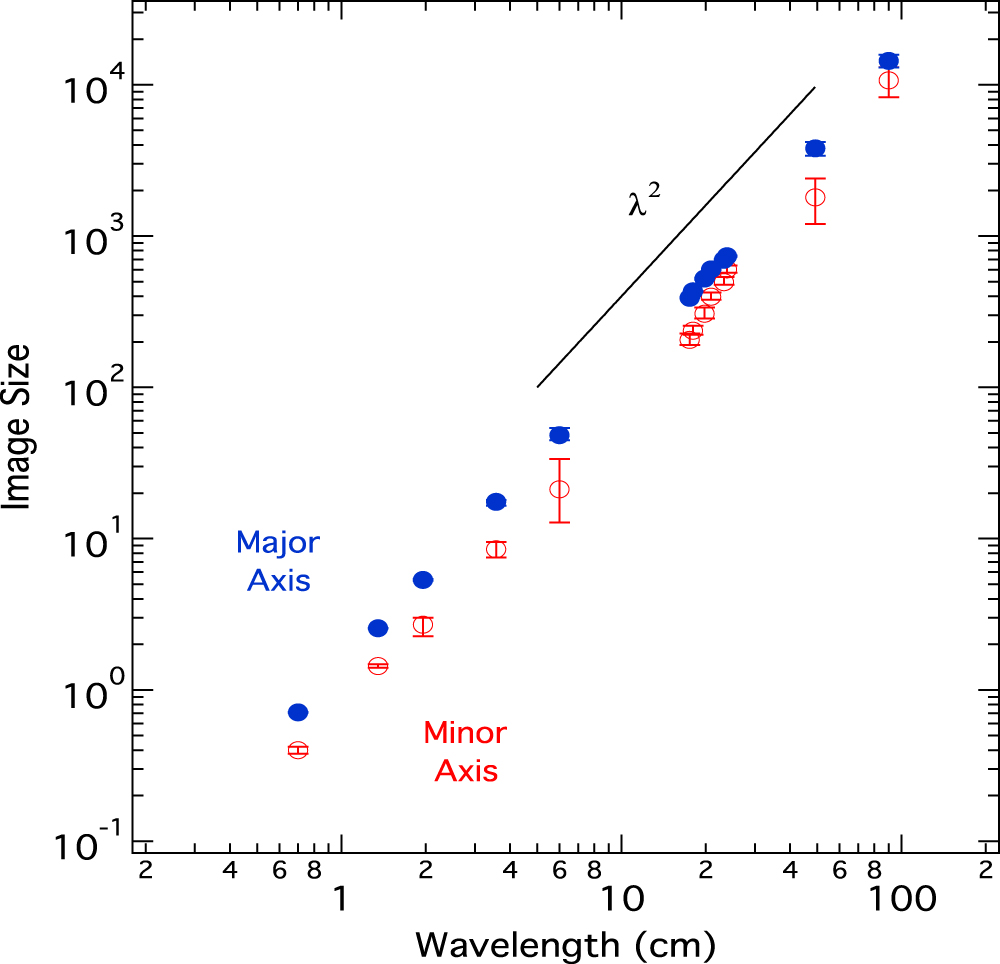
\includegraphics[width=0.6\columnwidth]{Images/scattering_law}
\caption{The $\lambda^2$ dependence of scattering kernel size is shown by the solid line. This has been derived from measurements made at $\lambda > 17$~cm \cite{Bower_2006}. The dotted line shows the derived intrinsic source size which scales as $\lambda^1.44$. This was derived from measurements in the wavelength range, 2~cm~$< \lambda < 1.3$~mm. The red circles show major-axis observed sizes of Sgr~A$^\star$  and the green points show the derived intrinsic major-axis size. This plot was reproduced from \citet{Doeleman_2008}.\label{fig:scattering_law}
}
\end{center}
\end{figure*}
%table showing latest scattering kernel parameters
\begin{table}[]
\centering
\caption{A re-analysis of VLBI observations of Sgr~A$^\star$ by \citet{Psaltis_2015} has yielded revised estimates of the parameters associated with the Gaussian scattering kernel. An accurate estimation is needed for accurate extrapolation to 1.3~mm. Note that the position angle is measured East of North. \label{tab:ism_gauss}}
\begin{tabular}{l|ll}
\hline
major axis FWHM (mas/cm$^-2$)& 1.32 & 0.04 \\
minor axis FWHM (mas/cm$^-2$)& 0.82 & 0.21 \\
position angle ($^\circ$)& 77.8 & 9.7\\  
\hline
\end{tabular}
\end{table}


%theory - refractive scale and size of blurred image
The Gaussian blurring effect can explained by the simple scattering model introduced in  Sec.~\ref{sec:basic_scat}. Recall, that in the strong scattering regime light is propagated from coherent patches with linear size $\sim r_0$. Each patch will emit light coherently into a single-slit diffraction cone of angular size $\theta_{\rm scatt} \sim \lambda /r_0$. An observer will hence be illuminated by many patches spanning $\theta_{\rm scatt}$, yielding a blurred and broadened image, with projected size on the screen equal to the \emph{refractive scale} 
$$r_{\rm ref} = \theta_{\rm scatt} D_{\rm os} = r_{\rm F}^2/r_0.$$
$r_{\rm ref}$ is the third fundamental length scale in the strong scattering regime and is associated with the refractive timescale,
$$t_{\rm ref} = r_{\rm ref}/v.$$
%calculating r_0 given \theta_scatt 
We can calculate $r_0$ given the FWHM of $\theta_{\rm scatt}$ through the more precise relation
\begin{equation}\label{eq:theta_scatt}
 \theta_{\rm scatt} = \frac{2\sqrt{2\ln{2}}}{2\pi} \lambda / r_0 (M+1)
\end{equation} 
where $M = D_{\rm os}/R$ is the magnification and $R$ is the source-screen distance. The magnification factor is a correction to the model introduced in Sec.~\ref{sec:basic_scat} when $R \sim \infty$ no longer holds and should be used when calculating distances in the observer plane \citep*{Goodman_1989}.
%Locating the scattering screen Bower 2014
The location of the scattering medium was originally thought to be quite close to Sgr~A$^\star$. However, observations of a newly discovered pulsar, SGR~J1745-29, indicate that the scattering screen is located at a distance $D_{\rm os} = 5.8 \pm 0.3$~kpc, within the Scutum spiral arm. Using Eq.~\ref{eq:theta_scatt} and the parameters given in table \ref{tab:ism_gauss}, we find that the major axis of the coherence length at 1.3~mm, $r_0 \approx 3136.67$~km.


%shift to looking at refractive effects,theory, 3 regimes of scattering
As the VLBI moves to higher frequencies, focus has shifted away from the well-studied Gaussian convolution effect of ISM scattering and onto the presence of stochastic scattering-induced substructure. To understand this phenomenon, we must first develop our conceptual framework. 

Strong scattering can be further subdivided into \emph{snapshot}, \emph{average} and \emph{ensemble-average} regimes \citep*{Narayan_1989,Goodman_1989}. To understand the different regimes, remember that for each point on the source, the observer sees emission from coherent patches of size $\sim r_0$ spanning $\sim r_{\rm ref}$. The diffraction cones from each of the patches will interfere, resulting in a multi-slit \emph{diffractive scintillation} pattern. 

%snapshot regime
In the \emph{snapshot regime}, a compact source is observed with a narrow bandwidth and over a short time integration. This yields a single realisation of the diffractive scintillation pattern. By averaging over many snapshots, diffractive scintillation is quenched. This occurs if the source size $\theta_{\rm src}$ is much larger than the diffractive scale $\theta_{\rm src} \gg r_0/R$; if the fractional bandwidth $\delta \nu/\nu$ is much larger than the decorrelation bandwidth $\delta \nu/\nu \gg \delta \nu_{\rm dc}/\nu \approx (r_0/r_{\rm F})^2$ \citep{Narayan_1992}; or if the integration time $t_{\rm int}$ is much larger the diffractive timescale $t_{\rm int} \gg t_{\rm 0} = r_0/v$, where $v$ is the relative velocity between screen, source and observer. This regime is hence only accessible through observations of compact objects like pulsars. On a side note, observations in this regime can be used to probe the source with angular resolution given by the $\sim \lambda /r_{\rm ref}$ \citep[e.g.][]{Gwinn_2012}. This is because the scattering screen is essentially a lens of size $\approx r_{\rm ref}$.

%average regime 
In the \emph{average regime}, diffractive scintillation has been averaged over, however there still exists scintillation over scales comparable to the size of the scattered image of a point source $\sim r_{\rm ref}$, termed \emph{refractive scintillation}. Phase fluctuations on this scale acts like a weak lens to focus or defocus the $\lambda/ r_0$ scale diffraction cones in the direction of the observer. For a point source this would lead to weak flux variations in the total flux \citep{Narayan_1992}. We will show later that refractive scintillation leads to the presence of substructure for a resolved scatter-broadened source. In contrast to diffractive scintillation, refractive scintillation is much more difficult to average over. Typically the refractive time scale $t_{\rm ref} = r_{\rm ref}/v$ is on the order of weeks to months for Sgr~A$^\star$; the fractional decorrelation bandwidth is on the order of unity $\delta \nu_{\rm dc}/\nu \sim 1$; and the source has to be much larger than the image of a scattered point source $\theta_{\rm src} \gg \theta_{\rm scatt}$. 

%ensemble average
In the \emph{ensemble-average regime}, both diffractive and refractive scintillation have been averaged over. It is in this regime when  the scattering is equivalent to Gaussian convolution which is deterministic and not time variable. 


%approximation of the scattered image by Johnson 2015
A recent theoretical work \citep*{Johnson_2015a} has derived a useful approximation of the resolved scattered image $I_{\rm ss}$ in the average regime,
\begin{equation}\label{eq:scatterbrane}
I_{\rm ss}(\mathbf{x}) \approx I_{\rm src}\left(\mathbf{x} + r_{\rm F}^2 \nabla \phi(\mathbf{x})\right),
\end{equation}
where $\nabla$ is the directional derivative. Here we have used the same two-dimensional coordinate system, indexed by $\mathbf{x}$ to describe the source, screen and observer planes which are considered to be aligned along the vertical axis. The scattered image $I_{\rm ss}$ is approximated by a 'reshuffling' of the source image $I_{\rm src}$. As $|\nabla\phi| \sim 1/r_0$, the magnitude of the translation of points on $I_{\rm src}$ $\sim r_{\rm ref} \sim 10\ \mu$-arcsec in the case of Sgr~A$^\star$. 

%Coherence of the phase slope
Even though $\phi(\mathbf{x})$ is only coherent to $\sim r_{\rm 0}$, the directional phase derivative $\nabla \phi(\mathbf{x})$ remains spatially coherent over much larger scales. Following \citet*{Johnson_2015a}, the autocovariance of phase derivative can be related to the structure function
\begin{align}
\langle [ \partial_x \phi(\mathbf{x_0})] [ \partial_x \phi(\mathbf{x_0}+\mathbf{x})] \rangle &=\
-\partial^2_x \langle \phi(\mathbf{x_0}) \phi(\mathbf{x_0}+\mathbf{x}) \rangle \\
&= \partial_x^2 D_\phi(\mathbf{x}).
\end{align}

as $\langle \phi(\mathbf{x})^2 \rangle = 0$

Using a typical structure function \citep{johnson_dissertation},We are interested in the case $r_{\rm in} \gg r_0$, the structure function becomes \citep{johnson_dissertation}
\begin{equation*}
D_\phi =
\begin{cases}
\left( \frac{r}{r_0}\right)^2 & \text{if } r \ll r_{\rm in},\\
\frac{2}{\beta}\left( \frac{r_{\rm in}}{r_0}\right)^{2-\beta} \left( \frac{r}{r_0}\right)^\beta & \text{if } r \gg r_{\rm in}.
\end{cases}
\end{equation*}

Note that the structure function is quadratic at small scales as fluctuations are smooth andthen kolmogorov then constant (Tatarskii, 1971).
Hence We are interested in the case $r /gg r_{\rm in}$
\begin{equation}
\partial_x^2 D_\phi(\mathbf{x})= \left(\frac{r_{\rm in}}{r_0}\right)^{2-\beta}  2(\beta -1)  \frac{r^{\beta-2}}{r_0^\beta}
\end{equation}

Therefore in the Kolmogorov regime $\beta = 5/3$, the coherence of image shift relative to the refractive scale $\propto (r/r_0)^{-1/3}$. Inner scale extends coherence and outer scale cuts it off.

%ESTIMATE OF COHERENCE .. awaiting discussion with roger 

If $\nabla \phi(\mathbf{x})$ was incoherent between patches of size $\sim r_0$, this would effectively be convolution with Gaussian of size $r_{\rm ref}$. 
)

%Observations of substructure

A recent observation of Sgr~A$^\star$ at 3.5~mm by the VLBA+LMT \citep[see Fig.~ref{fig:substructure2}][]{Ortiz_2016} show that the closure phase measured is consistent with refractive scintillation. Another observation at 1.3~cm shows flux modulation due to scattering substructure $\sim 10$~mJy \citep{Gwinn_2014} and other predictions show $\sim 60$~mJy for long East-West baselines and $\sim 25$~mJy for long North-South baselines \citep*{Johnson_2015a}, assuming a Gaussian source of $FWHM=40\ \mu$-arcsec.

\begin{figure*}
\begin{center}
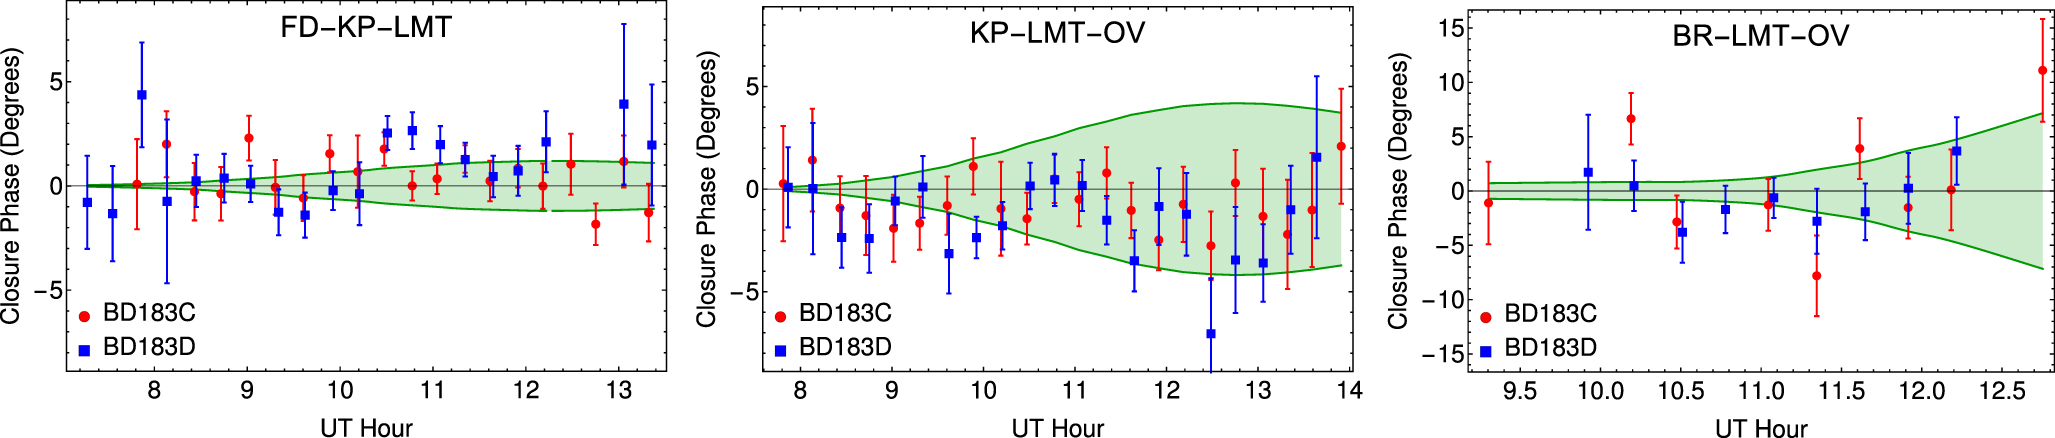
\includegraphics[width=\columnwidth]{Images/ism_cp}
\caption{Closure phases recorded in a VLBA + LMT observation of  Sgr~A$^\star$ at $\lambda = 3.5$~mm \cite{Ortiz_2016}. The data points are shown as red circles and blue squares and are only distinguished by the calibrator used. The green envelopes show the $1\sigma$ closure phase prediction induced by scattering-induced substructure. Reproduced from \citet{Ortiz_2016} \label{fig:substructure2}
}
\end{center}
\end{figure*}


%Distinguishing intrinsic source structure and variability
Distinguishing intrinsic source structure and variability and ISM variability is an interesting challenge. Observations at mm-wavelengths have revealed deviations from the $\lambda^2$ scattering scaling law, see Fig.~\ref{fig:scattering_law}. This is interpreted as due to the presence of intrinsic source structure and has been fitted with a power-law with an exponent of $1.34 \pm 0.01$ \cite{Lu_2011}. This has enabled the constraint of various theoretical models \cite{Bower_2006}, excluding advection-dominated accretion flows (ADAF) \cite{Narayan_1998} and Bondi-Hoyle accretion \cite{Melia_1994}. However observations extending over month timescales are required to properly sample the larger scale inhomogeneities and even with multiple epoch observations, it can be difficult to distinguish source and scattering characteristics \citep*{Macquart_2006}.

Knowledge of the scattering characteristics can allow the two to be decoupled without sampling a refractive ensemble. It therefore provides
a robust and rapid mechanism for quantifying refractive effects.



\subsection{Troposphere}
%PR 1 St 1

%Introduction - Troposphere is a problem. Define troposphere. st 1
The coherence and intensity of millimetre wavelength electromagnetic waves are most severely deteriorated in the lowest atmospheric layer, the troposphere which extends up to an altitude of $7-10$~km above sea level and down to a temperature $T \sim 218$~K \citep{Thompson_2001}. The troposphere is composed of a number of different components including primary gases $\rm N_2$ and  $\rm O_2$, trace gases e.g. water vapour and ${\rm CO_2}$, as well as particulates of water droplets and dust. The rest of this section will explore the tropospheric corruption for the mm-VLBI case. 


\subsubsection{Propagation fundamentals}
%propagation fundamentals st 1
Consider a quasi-monochromatic wave passing through a linear medium,
\begin{equation}
E_\nu(x,t) = E_0 \exp^{i(kn_\nu x - 2\pi\nu t)},
\end{equation}		
where $k=2\pi \nu/c$ is the propagation constant in free space and $n= n_{\rm R} + j n_{\rm I}$ is the complex index of refraction. Note that we will occasionally omit the frequency dependence of $n$ and related quantities to simplify the notation. If $n_{\rm I}$ is nonzero, the electric flux $I$ will decay exponentially
\begin{equation}
I = EE^\ast = E_0^2 \exp(-\tau),
\end{equation}
where $\tau$ is called the opacity or optical depth and is related to the absorption coefficient, $d\tau = \kappa dx$ where $\kappa = 4\pi \nu n_I/c$. If $n_{\rm R} > 1 $ the phase velocity of light will decrease, $v_{\rm p} = c/n_{\rm R}$, which results in a time delay. The time delay, $\delta t$ and opacity $\tau$ can be calculated simultaneously,
\begin{equation}\label{timedelay}
\delta t + i \tau /4\pi \nu =1/c \int_{path} d\mathbf{s}\  (n_\nu(\mathbf{s}) -1).
\end{equation}

%the relationship between delay-absorption-noise st 1
In the interferometric context opacity and time delay are often viewed independently. However, the electric field is real and causal which imposes restrictions on the complex refractive index. Specificially $n_{\rm R}$ and $n_{\rm I}$ contain the same information and can be interchanged via the Kramers-Kronig relations. 

Absorption is accompanied by emission and for a medium in local thermodynamic equilibrium, Kirchoff's law states that 
\begin{equation}\label{kirchoff}
\frac{\epsilon_\nu}{\kappa_\nu}=B_\nu(T),
\end{equation}
where $\epsilon_\nu = dI_\nu/dx$ is the emission coefficient and $B_\nu(T)$ is the Planck function. Hence the absorbing molecules are also emitters, increasing system noise. Therefore opacity, time delay and atmospheric noise are interrelated and should be simulated consistently. On a side note these relations allow for phase calibration using measurements of sky emission via Water Vapour Radiometry (WVR) \citep*[e.g.][]{Carilli_1999}.

\subsubsection{Atmospheric corruptions in the (sub-)mm regime}
%st 1
%Absorption in the GHz regime st 1
An analysis of the absorption spectrum in the GHz range (Fig.~\ref{fig:absorption}), shows that it is dominated by transitions of $\rm H_2O$ and $\rm O_2$ as well as a pseudo-continuum opacity which increases with frequency. The pseudo-continuum opacity is due to the cumulative effect of the far wings of a multitude of broadened water vapour lines above 1~THz \citep{Carilli_1999}. At 230~GHz the absorption is typically $5-10$\% at the best sites, during good weather. 

%Fig Absorption spectrum in the GHz st 1
\begin{figure*}
\begin{center}
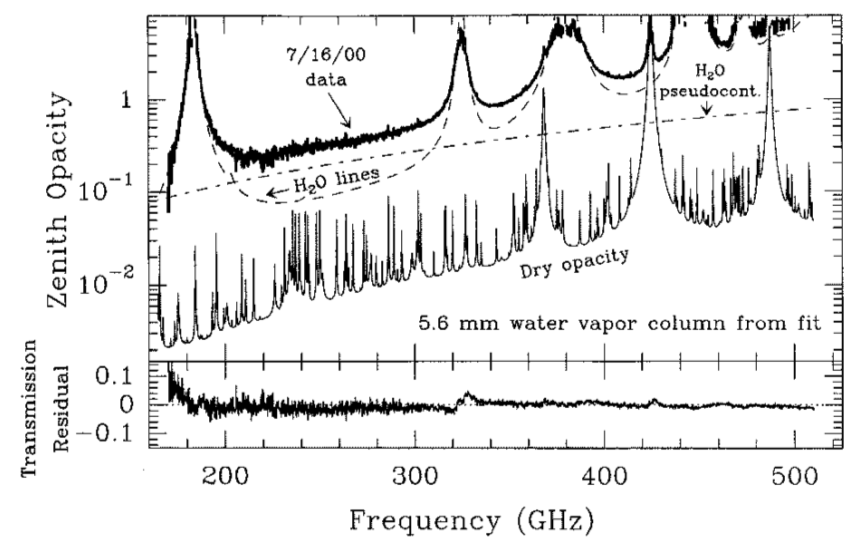
\includegraphics[width=\columnwidth]{Images/absorption}
\caption{Recorded zenith absorption spectrum in the $160-520$~GHz range, taken on Mauna Kea at an altitude of $\sim 4000$~m. The data has been fit to a sum of $\rm H_20$ lines, an $\rm H_20$ pseudo-continuum and dry absorption lines. The model has been generated using the \textsc{atm} code, with the bottom panel showing the residuals. Here 'dry' refers to all atmospheric constituents except $\rm H_20$. Reproduced from \citet{Pardo_2001} \label{fig:absorption}
}
\end{center}
\end{figure*}

%Phase variability in the GHz st 1
In contrast to the dry atmospheric components, water vapour mixes poorly and its time-variable spatial distribution induces rapid fluctuations in the time delays $\delta t (\nu)$ above each station. The phase error for a baseline (1,2) where antenna 1 is the reference will be
\begin{equation}
\delta \phi(t, \nu) = (\delta t_2(t, \nu) - \delta t_1(t, \nu))/\nu.
\end{equation}
The water vapour column density is measured as the depth of the column when converted to the liquid phase and is referred to as the precipitable water vapour (PWV). PWV is directly proportional to the time delay and hence the phase delay, 
\begin{equation}
\delta\phi \approx \frac{12.6\pi}{\lambda} \times w, 
\end{equation}\label{eq:phi-pwv}

\noindent where $w$ is the depth of the PWV column \citep*{Carilli_1999} and an atmospheric temperature $T=270$~K has been assumed. This relationship between phase and water vapour content has been experimentally verified \citep{hogg_1981}. At 230~GHz, the change in PWV needed to offset the phase by 1~rad is $\Delta w\approx0.03$~mm. 

This sensitive dependence of phase coherence on atmospheric stability is aggravated by typically low antenna observation elevation angles as the atmospheric path length is increased; uncorrelated atmospheric variations between stations as correlated atmospheric variations fall away; and observing with a sparse VLBI array as this leads to less redundancy for calibration.


\subsubsection{Radiative transfer}\label{sec:atm_theory}
%St 1

%Radiative transfer, how solving it will give observables in a self-consistent manner st 1
The problem of radiative transfer through the Earth's atmosphere is well described and implemented by the Atmospheric Transmission at Microwaves (\textsc{atm}) description and code \citep{Pardo_2001}. In this section we provide a brief summary of the theory underpinning the package and we encourage the reader to see the original paper for further detail. The incorporation of {\sc atm} into the {\sc MeqSilhouette} simulator is dealt with in section~\ref{sec:trop_imp}. \textsc{atm} is commonly used in the Atacama Large Millimeter Array (ALMA) community \citep{Curtis_2009,Nikolic_2013} and has been tested with atmospheric transmission spectra taken on Mauna Kea \citep{Serabyn_1998}.

%Radiative transfer st 1
We start from the unpolarised radiative transfer equation, which is unidirectional in the absence of scattering,
\begin{equation}\label{eq:rad_trans}
\frac{dI_\nu (s) }{ds} = \epsilon_\nu(s) -\kappa_\nu(s)  I_\nu (s),
\end{equation}
where $s$ is the coordinate along the signal path through the atmosphere.  The assumption of local thermodynamic equilibrium (LTE) holds as the collisional timescale is much smaller than the time for spontaneous emission up to altitudes $\ge 80$ km, after which there is only $\sim 0.001\%$ of mass left \citep{Pardo_2001}. Applying \ref{kirchoff}, multiplying by $\exp(-\tau_\nu)$ and integrating from the top of the atmosphere ($s=0$) yields, 
\begin{equation}\label{eq:rad_trans2}
I_\nu(s) = I_\nu(0) e^{-\tau_\nu (0,s) }+ \int_0^s B_\nu(s')e^{-\tau_\nu (s',s) }\kappa_\nu(s')ds',
\end{equation}
where  $s'$ is a dummy variable in the same direction as $s$ and $\tau_\nu (0,s) = \int_0^{s} k_\nu(s')ds'$. $I_\nu(0)$ is normally taken as the radiance from the cosmic background.
\ref{eq:rad_trans2} will allow us to calculate the noise temperature of the atmosphere by converting the output radiance at the ground $I_\nu(s)$ to  the equivalent blackbody temperature through inversion the Planck function. To calculate the opacity and complete the above integral, $\kappa_\nu$ needs to be calculated over the frequency range. The time delay $\delta t$ can be calculated using the Kramers-Kronig relations. 


%deriving the absorption coefficient st 1
A general equation for the absorption coefficient for a transition between a lower $l$ and upper $u$ states is given in the original paper. Here we merely point out that it should be proportional to the energy of the photon, $h\nu_{l \to u}$, the transition probability or Einstein coefficient, $ B_{l \to u}$, the line-shape, $f(\nu,\nu_{l \to u})$ and the number densities $N$ of electronic populations. Line profiles which describe pressure broadening (perturbations to the Hamiltonian due to the presence of nearby molecules) and Doppler broadening are used. The condition of detailed balance further requires that decays from the upper state are included yielding, $g_u B_{u \to l} =g_l B_{l \to u}$, where $g$ is the degeneracy of the electronic state. Putting this together we find,

\begin{equation}
\kappa(\nu) _{l \to u}  \propto  h\nu   B_{l \to u}  \left(\frac{N_l}{g_l}  -  \frac{N_u}{g_u} \right) f(\nu,\nu_{l \to u}),
\end{equation}

\noindent where the Einstein coefficients are calculated from the inner product of the initial and final states with the dipole transition operator, 
\begin{equation}\label{coefficient}
B_{l \to u} = \frac{2\pi}{3\hbar^2} |<u|\mu|l>|^2,
\end{equation}
where $|u>$, $|l>$,$|\mu>$ are the wavefunctions of upper and lower states and the dipole transition operator respectively.
The number densities of the two states, $N_u$ and $N_l$ in local thermodynamic equilibrium (LTE) are simply related to the local number density and temperature via Boltzmann statistics,
\begin{equation}
\frac{N_n}{N} = g_n \frac {\exp{-\frac{E_n}{kT}}}{Q}
\end{equation}
where Q is the partition function. $Q = \sum_i g_i  \exp{-E_n/kT}$. 

%lineshapes and pseudocontina st 1
Physically, the lineshape originates from perturbations to the hamiltonian due to proximity to neighbouring molecules, called pressure broadening, and at lower pressures, thermal doppler broadening. A Van Vleck -Weisskopf (VVW) profile is used for pressure broadening. At lower pressures this is convolved with a Gaussian which arises from the Maxwellian distribution. 
Far wing broadening of $H_2O$ lines $> 1.2$ THz extends to lower frequencies and is not completely represented by the VVW profile. This is believed to be due to self-self collisions of water molecules. Additionally there are terms from the dry atmosphere related to transient dipoles and Debye absorption which are not represented in the lineshape. To correct for these effects two pseudocontina are used, which take the form of a power law dependence on frequency, temperature and the molecular densities. 

%inner product st 1
Transition lines at radio wavelengths result from rotational state transitions. To calculate the inner product given in equation~\ref{coefficient}, hamiltonians for linearly symmetric rotors (e.g. $O_2$, $CO$) and asymetric rotors are used. The asymetric rotations are decomposed into three principal rotation axes with differing rotational constants governing each axis. Rotational constants were measured by the authors as well as drawn from a variety of literature. Partition functions and transition probability are calculated using approximations taken from the literature.


\subsubsection{Turbulent phase fluctuations}\label{sec:turb_theory}
%St 1

%phase fluctuations as a calibration problem st 1
Visibility phase instability  $\delta \phi(t)$ due to tropospheric turbulence is a fundamental limitation to producing high fidelity, science-quality maps with a mm-VLBI array \citep{Thompson_2001}. The coherence time-scale is typically too rapid ($\lesssim10$~s) for fast switching calibration, so other calibration procedures (e.g. water vapour radiometry, paired antennas, and/or self-calibration) must be performed. Self-calibration is the most commonly used but is limited by the integration time needed to obtain adequate SNR to fringe fit. Phase decoherence often leads to the use of closure quantities to perform model fitting \citep{Doeleman_2001,Bower_2004, Shen_2005}, and causes a decrease in measured flux due to incoherent complex averaging.
%plan
In the section we will review and develop the weak scattering theory introduced earlier which will culminate in a formulation for the simulation of tropospheric phase turbulence seen by a mm-VLBI array. How this formulation is implemented and fits into the broader atmospheric simulation framework will be discussed in section~\ref{sec:trop_imp}. 


%Following from scattering intro, weak scattering model setup st 1
Following from section~\ref{sec:basic_scat}, we can model the statistics of $\delta \phi(t)$ with a thin, frozen, Kolomogorov-turbulent phase screen moving with a bulk velocity, $v$.  We set the height $h$ of the screen at the water vapour scale height of 2~km above ground. We will show later that the thickness $\Delta h$ of the atmospheric turbulent layer can be neglected in our implementation. At $1.3$~mm, the Fresnel scale is $r_F \approx 0.45$~m and experiments show annual variations of $r_0 \sim 50 - 500$~m above Mauna Kea \citep{Masson_1994} and $r_0 \sim 90 - 700$~m above Chajnantor \citep*{Radford_1998}, where both sites are considered to have excellent atmospheric conditions for millimetre astronomy. As $r_F < r_0$, this is an example of weak scattering. 


%simplifying the scattering model st 1
The required field-of-view (FoV) of a global mm-VLBI array is typically FoV~$< 1$~mas or ~$\sim10~\mu$m at a height of 2~km, which is roughly 7-8 orders of magnitude smaller than the tropospheric coherence length. The tropospheric corruption can therefore be considered constant across the FoV and, from the perspective of the Measurement Equation, modeled as a diagonal Jones matrix per time and frequency interval. As VLBI baselines are much longer than the coherence length, $|\mathbf{b}| \ge 1000$~km~$\gg \rm r_0$, the phase screen at each site must be simulated independently. This assumption only holds for VLBI baselines and the framework needs to be extended to simulate the effects of turbulence on individual phased arrays stations (e.g. SMA) and short ($<10$~km) baselines (e.g. JCMT - SMA). 

%structure function formulation st 1
Our aim then is to produce a phase error time sequence $\left\{\delta \phi(t_i)\right\}$ for each station which is added to the visibility phase. We invoke the frozen screen assumption and write the structure function as a function of time, $D (t) =  D(r)|_{r=vt}$. The temporal structure function $D(t)$ provides an efficient route to sample the variability of the troposphere at the typical integration time of the dataset, $t_{\rm int} \sim 1$~sec. 

The temporal variance of the phase is a function of the temporal structure function, and accounting for time integration yields \citep*[see][B3]{Treuhaft_1987} 

\begin{equation}
\sigma^2_{\phi}(t_{\rm int}) = (1/t_{\rm int})^2 \int_{0}^{t_{\rm int}} (t_{\rm int}-t) D_{\phi}(t) dt.
\end{equation}

Assuming power-law turbulence and integrating yields, 

\begin{equation}\label{eq:turb_final}
\sigma^2_\phi (t_{\rm int})=\left[\frac{1}{\sin\theta(\beta^2 +3\beta +2)}\right]\left(\frac{t_{\rm int}}{t_0}\right)^{\beta},
\end{equation}


\noindent where $t_0 = r_0/v$ is the coherence time when observing at zenith and $1/\sin\theta$ is the approximate airmass which arises as $D_\phi \propto w$. As $r \ll \Delta h$, where $\Delta h$ is the thickness of the turbulent layer, an thin screen exponent of $\beta = 5/3$ is justified \citep*{Treuhaft_1987}. The phase error time-series takes the form of a Gaussian random walk per antenna. At mm-wavelengths, the spectrum of water vapour is non-dispersive up to a few percent \citep{Curtis_2009} and so we can assume a simple linear scaling across the bandwidth.



%Fig. Phase variability carilli_1997 st 1
\begin{figure*}
\begin{center}
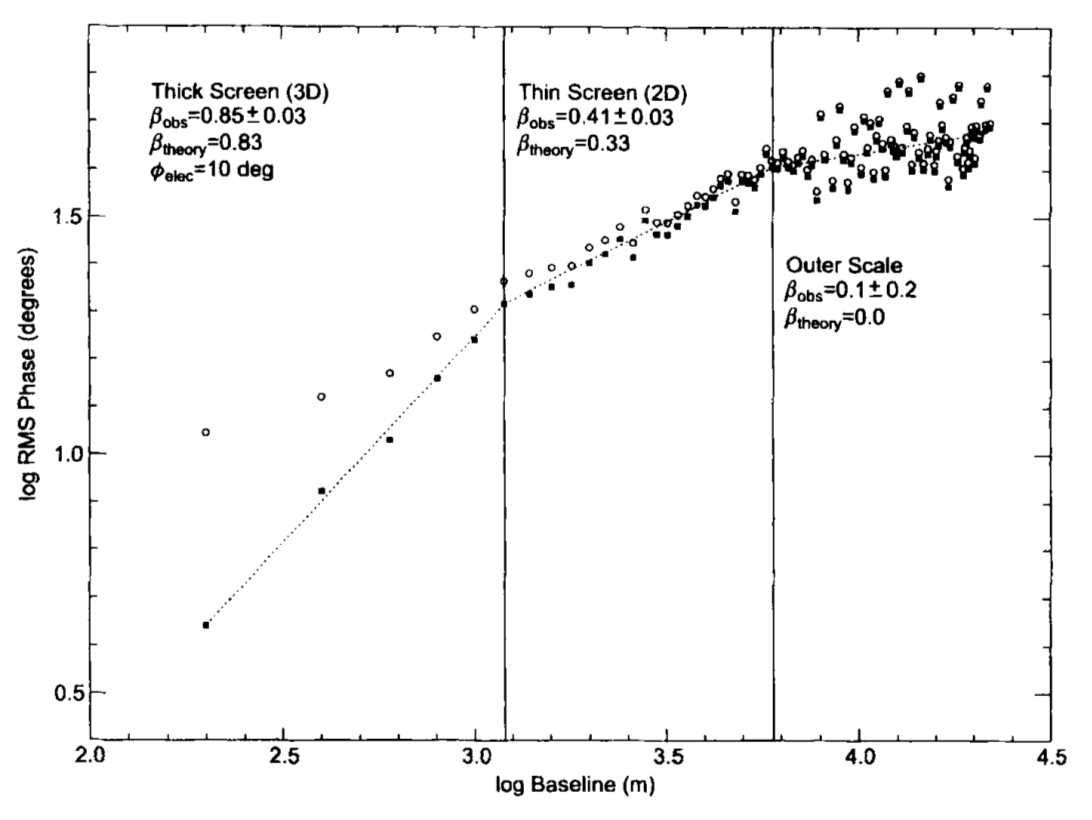
\includegraphics[width=\columnwidth]{Images/screentransition}
\caption{A log-log plot of RMS visibility phase versus baseline length for an observation of 1~Jy source 0748~+~240 with VLA at 22~GHz over a 90~min duration. The open circles show RMS phase as measured whereas the solid squares show the same values with a constant thermal noise contribution of $10^\circ$ subtracted in quadrature. Note that the measured and theoretical Kolmogorov turbulent exponent $\beta$ changes with distance on the phase screen as the viewing configuration transitions from a thick screen ($\beta_{\rm theory} = 5/3$) to a thin screen ($\beta{\rm theory = 2/3$) at $r \approx 1.2$~km and from a thin screen to completely uncorrelated regime ($\beta = 0$) beyond the outer scale at $r \approx 6$~km. Although these regimes appear distinct, there is continous variation between them. Reproduced from \citet{Carilli_1997} \label{fig:screentransition}
}
\end{center}
\end{figure*}


%A comparison to the phase screen approach st 1
Phase fluctuations $\delta\phi(t)$ can also be simulated by taking the inverse Fourier transform of the spatial phase power spectrum. However this approach is much more computationally expensive, e.g. for an observation length $t_{\rm obs}$ involving $N_{\rm ant}=8$ independent antennae with dish radii $r_{\rm dish}=15$~m, wind speed $v=10$~m\,s$^{-1}$ and pixel size equal to $r_{\rm F}$, the number of pixels $N_{\rm pix} \approx N_{\rm ant} t_{\rm obs} r_{\rm dish}^2/(v r_{\rm F}^3)  \sim 10^8$. Additionally, due to fractal nature of ideal Kolmogorov turbulence, the power spectrum becomes unbounded as the wavenumber approaches zero which makes it difficult to determine the sampling interval of the spatial power spectrum \citep{Lane_1992}. 


\subsection{Instrumental}

\subsubsection{Thermal Noise}
%Pr 1 St 1

%Mild derivation of the thermal noise equation.
The  level of thermal noise in the data will define the sensitivity of the interferometer to detect a source and also to distinguish fine source characteristics. Closure quantities are especially prone to high levels of thermal as several visibilities are multiplied. A derivation of the thermal noise of an interferometer can be made through derivation of the thermal noise of an antenna and then correlating the result \citep*{Wrobel_1999}. The RMS thermal noise of an interferometer $\{i,j\}$ over a bandwidth $\Delta \nu$ and an integration time is given by 

\begin{equation}
 \Delta S_{\rm ij} = \frac{1}{\eta_{\rm s}}\sqrt{\frac{SEFD_{\rm i}\ SEFD_{\rm j}}{2 \Delta \nu t_{\rm int}}},  
\end{equation}
where $\eta_{\rm s}$ is the system efficiency and $2 \Delta \nu t_{\rm int}$ is the number of independent samples. The $SEFD$ is a measure of the sensitivity of an antenna, accounting for the effiency, collecting area and thermal noise and is defined as the flux density of a source with the same power,
\begin{equation}
 SEFD = 2 k_{\rm B} T_{\rm sys} / (\eta_{\rm a} A),
\end{equation}
where $A$ is the antenna area, $\eta_{\rm a}$ is the antenna efficiency, $T_{\rm sys}$ is the system temperature and the factor $\frac{1}{2}$ accounts for only sampling 1 polarisation.


\subsubsection{Antenna Pointing}
%Pr 1 St 1
%Intro
All antennas suffer pointing errors to some degree due to a variety of factors including dish flexure due to gravity, wind and thermal loading, as well as drive mechanics. This corresponds to an offset primary beam, which should only translate to minor amplitude errors if the pointing error $\theta_{\rm PE}$ is significantly smaller than the primary beam (i.e. $\theta_{\rm PE} \ll \theta_{\rm PB}$). In the Measurement Equation formalism, this offset can be represented by a modified (shifted) primary beam pattern in the {\bf \it E}-Jones term 
\begin{equation}
{\bf E}_p(l,m) = {\bf E}(l_0 + \delta l_p, m_0 + \delta m_p),
\end{equation}
where $\delta l_p, \delta m_p$ correspond to the directional cosine offsets.
%Motivation, why this could be a problem for mm observations
This could be a problem for millimetre observations as the primary beam is significant, e.g. for a 30~m dish at 1.3~mm, $\theta_{\rm PB} \sim 10$~arcsec, compared to the pointing error which is on the order of arcseconds.
%beam shape
A standard beam model which we will make use of later is the analytic WSRT beam model \citep{Popping_2008} 
\begin{equation}
E(l, m) = \cos^3(C\nu \rho),\qquad   \rho = \sqrt{\delta l_p^2 + \delta m_p^2}
\end{equation}
where $C$ is a constant, with value $C \approx 130$~GHz$^{-1}$. Note that the power beam $EE^H$ becomes $\cos^6$. 
% Different categories of pointing error i.e. tracking vs slew

An antenna tracking a source will suffer a slow, continuous time-variable pointing error associated with the tracking error $\sigma_{\rm track}$. Physically this could be attributed to changes in wind, thermal and gravitational loading which all change with telescope pointing direction and over the course of a typical few hour observation. Using the MeqTrees software package, such behaviour has been demonstrated to occur with the Westerbork Synthesis Radio Telescope (WSRT, \cite{Smirnov_2011c})\footnote{See also https://indico.skatelescope.org/event/\\171/session/9/contribution/20}.


Whilst a stationary phase centre is tracked, the pointing error should evolve slowly and smoothly, however, in mm-VLBI observations the phase centre is often shifted to another source/calibrator. This would cause the pointing error to change abruptly, with an absolute pointing error $\sim \sigma_{\rm abs}$. Source/calibrator change is scheduled every 5-10 minutes in a typical millimetre observation. The point is that even though EHT will be able to determine the pointing offset when observing a calibrator with well known structure, when the antennas slew back to a source (e.g. Sgr~A$^\star$) with less certain or variable source structure, the pointing error could change significantly. This is exacerbated by the scarcity of mm-wavelength calibrators, which are often widely separated from the source.
